\lab{Numerical Differentiation}{Numerical Differentiation}
\label{lab:NumericalDerivatives}
\objective{The derivative is exceptionally useful in many applications, but we often do not know the original function or the derivative may be too difficult to compute. In these situations, finite difference quotients are beneficial to use to approximate the derivative. In this lab, we will implement several methods for approximating the derivative of a function numerically. Additionally, we will explore the accuracy of these approximations with respect to: the number of points used, the value of h and the number of dimensions. }
%
\section*{Derivative Approximations in One Dimension} % =======================
%
The derivative of a function $f$ at a point $x_0$ is
%
\begin{equation}
\label{eqn:deriv}
f'(x_0) = \lim_{h\rightarrow 0} \frac{f(x_0 + h)-f(x_0)}{h}.
\end{equation}
%
In this lab, we will investigate one way a computer can calculate $f'(x_0)$.
%
\subsection*{Forward Difference Quotient} % -----------------------------------
%
Suppose that in Equation \eqref{eqn:deriv}, instead of taking a limit, we just pick a small value for $h$.
$f'(x_0)$ is expected to be close to the quantity
%
\begin{equation}\label{equ:forward_diff}
\frac{f(x_0 + h)-f(x_0)}{h}.
\end{equation}
%
This quotient is called the \emph{first order forward difference approximation} of the derivative.
Using the points $x_0$ and $x_0-h$ in place of $x_0+h$ and $x_0$ respectively is called the \emph{first order backwards difference quotient}.
%
Because $f'(x_0)$ is the limit of such quotients, this quotient is close to $f'(x_0)$ when $h$ is small.
Taylor's formula shows just how close it is. By Taylor's formula,
\[
f(x_0+h) = f(x_0) + f'(x_0)h + R_2(h)
\]
where $R_2(h) = \left( \int_0^1 (1-t) f''(x_0+th) dt \right) h^2$
(this is the integral form of the remainder for Taylor's Theorem; see Volume 1 Chapter 6). When we solve this equation for $f'(x_0)$, we get
%
\begin{equation}\label{equ:forward_diff_with_remainder}
f'(x_0) = \frac{f(x_0+h)-f(x_0)}{h} - \frac{R_2(h)}{h}.
\end{equation}
%
Thus, the error in using the first order forward difference quotient to approximate $f'(x_0)$ is
\[
\left | \frac{R_2(h)}{h} \right | \leq |h| \int_0^1 |1 - t||f''(x_0+th)|dt.
\]
If we assume $f''$ is continuous, then for any $\delta$, set $M = \sup_{x \in (x_0-\delta, x_0+\delta)} f''(x)$. Then if $|h| < \delta$, we have
\[
\left | \frac{R_2(h)}{h} \right | \leq |h|\int_0^1 M dt = M|h|  {\in}  O(h).
\]
Similarly, the backward quotient is also in $O(h)$.
%
The \emph{second order forward difference quotient}, which uses three points $(x, x+h$, and $x+2h)$ instead of two, is given by:
%
\begin{equation}
f'(x_0)\approx\frac{-3f(x_0)+4f(x_0+h)-f(x_0+2h)}{2h}.
\end{equation}
And the \emph{second order backwards difference quotient}:
\begin{equation}
f'(x_0)\approx\frac{3f(x_0)-4f(x_0-h)+f(x_0-2h)}{2h}.
\end{equation}
%
\subsection*{Centered Difference Quotient}
%
A finite difference quotient that is in $ O(h^2)$, and consequently has a smaller error when $|h|<1$, is called the \emph{centered difference quotient}. It is defined for the second and fourth order respectively as:
\begin{equation}
f'(x_0)\approx\frac{f(x_0+h)-f(x_0-h)}{2h}
\end{equation}
\begin{equation}
f'(x_0)\approx\frac{f(x_0-2h)-8f(x_0-h)+8f(x_0+h)-f(x_0+2h)}{12h}.
\end{equation}
For a derivation of the second order centered difference quotient, please refer to the additional materials section.

\begin{problem}
In separate functions implement the
\begin{enumerate}
\item first order forward difference quotient,
\item second order backward difference quotient,
\item second order centered difference quotient, and the
\item fourth order centered difference quotient.
\end{enumerate}
Each function should accept a callable function $f$, an array of points, and a float representing $h$ that defaults to $10^{-5}$.
Return an array of the difference quotients.

To test your function, you can define a polynomial and calculate its derivative analytically.
Then pass your array of points into the analytically computed derivative and into your functions and verify that the returned arrays are close to one another.
\end{problem}
\subsection*{Accuracy of Approximations} % ------------------------------------

It is important to pick an appropriate step size $h$ when approximating a derivative by finite difference quotients.
The step size should be small but not too small, as dividing by very small numbers causes errors in floating point arithmetic.
This means that as we decrease $|h|$, the error $|f'(x_0)-\tilde{f}(x_0)|$ (where $\tilde{f}$ is the numerical approximation) will first decrease but then will increase as $|h|$ gets too small.

\begin{problem}
For the function $f(x) = (\sin(x)+1)^x$, calculate and plot the errors of the
\begin{enumerate}
\item second order backward difference quotient,
\item second order centered difference quotient, and the
\item fourth order centered difference quotient
\end{enumerate}
using your functions from Problem 1 to get the numerical approximations.
Do this for at least 6 evenly-spaced values of $h \in [10^{-8}, 1]$.
Use a \li{loglog()} plot, include a legend and put a dot on the graph for each value of $h$.
Your function should accept a float value where the derivative is being approximated at.

Hints: Define $f$ and analytically compute its derivative.
For each value of $h$, calculate and plot $|f'(x_0)-\tilde{f}(x_0)|$.
Consider using the NumPy function \li{logspace()} to define your $h$-values.
To include a point on your graph, put \li{'-o'} as an argument in your \li{loglog()} function call.

Evaluated at $x_0 = 1$, the plot of just the fourth order centered difference quotient should resemble Figure \ref{fig:errors}. You should notice a bend in each of the graphs, where the $h$-value is getting too small.

\begin{figure}[H]
\centering
\includegraphics[width=\linewidth]{error_plot.png}
\caption{The plotted errors of fourth order centered difference quotient for the function $f(x) = (\sin(x)+1)^x$ evaluated at $x=1$.}
\label{fig:errors}
\end{figure}

\end{problem}

\begin{warn}
Mathematically, choosing smaller h values results in smaller errors.
On a computer however, values of h that are too small result in imprecise computations due to \emph{catastrophic cancellation}, which we will discuss in Conditioning and Stability. Consequently, the optimal value of $h$ is one that is small but not too small, such as $10^{-5}$.
\end{warn}

Although the centered difference quotient gives a more accurate approximation of the derivative, there are some functions that do not behave well under centered difference quotients.
Additionally, information on both sides of the point $x_0$ may not be available.
In these cases, one must use the forward or backward difference quotient to approximate the derivative.

\begin{problem}
The radar stations A and B, separated by the distance a = 500 km, track a plane C by recording the angles $\alpha$ and $\beta$ at one-second intervals (See figure \ref{plane}).
Successive readings for $\alpha$ and $\beta$ at integer times $t \in [7, 14]$ are given in the textfile \texttt{plane.txt}.
The first column contains the integer values of t, the second contains the float values of $\alpha$ in degrees and the third contains the float values $\beta$ in degrees.
Use finite difference quotients to calculate the velocity of the plane for each value of $t$ in the file.
The coordinates of the plane are
\begin{equation}
x = a \frac{\tan(\beta)}{\tan(\beta)-\tan(\alpha)}
\end{equation}

\begin{equation}
 y = a \frac{\tan(\beta)\tan(\alpha)}{\tan(\beta)-\tan(\alpha)}.
\end{equation}

Use these functions to find the coordinates of the plane at each point in time and plot the trajectory (note that NumPy trigometric functions only accept angles in radians).  Then approximate $x'(t)$ and $y'(t)$ at each point (using the forward difference quotient on $t = 7$, the backward on $t=14$ and the centered on all other points). Plot the values of the velocity $\sqrt{x'(t)^2+y'(t)^2}$ at each point in time and then return them in an array.

The trajectory of the plane will be constantly increasing. And the values of the speed will vary between $.265$ and $.285$ km/sec which is approximately equivalent to $592-637$ mph.

(Kiusalaas, Jaan. Numerical Methods in Engineering with Python 3)
\end{problem}

\begin{figure}
\includegraphics[width=.5\textwidth]{figures/plane_diagram.png}
\caption{Radar stations in relation to plane}
\label{plane}
\end{figure}

\begin{info}
Finite difference quotients can be used to approximate higher-order derivatives of $f$.
However, taking derivatives is an unstable operation which can amplify the arithmetic error in your computation.
For this reason, difference quotients are not generally used to approximate derivatives higher than second order.
\end{info}

\section*{Derivative Approximations in Multiple Dimensions} % =================

Finite difference methods can also be used to calculate derivatives in higher dimensions.
Recall that the Jacobian of a function $f:\mathbb{R}^n \rightarrow \mathbb{R}^m$ at a point $x_0 \in \mathbb{R}^n$ is the $m \times n$ matrix $J = (J_{ij})$ defined component-wise by
\begin{equation*}
J_{ij} = \frac{\partial f_i}{\partial x_j}(x_0).
\end{equation*}
For example, the Jacobian for a function $f:\mathbb{R}^3 \rightarrow \mathbb{R}^2$ is defined by

\[
J = \begin{pmatrix}
\frac{\partial f}{\partial x_1}&\frac{\partial f}{\partial x_2}&\frac{\partial f}{\partial x_3}
\end{pmatrix}
= \begin{pmatrix}
\frac{\partial f_1}{\partial x_1}&\frac{\partial f_1}{\partial x_2}&\frac{\partial f_1}{\partial x_3}\\
\frac{\partial f_2}{\partial x_1}&\frac{\partial f_2}{\partial x_2}&\frac{\partial f_2}{\partial x_3}
\end{pmatrix}.
\]

The Jacobian is useful in many applications.  For example, the Jacobian can be used to find zeros of functions in multiple variables.

The forward difference quotient for approximating a partial derivative is
\begin{equation*}
\frac{\partial f}{\partial x_j} (x_0) \approx \frac{f(x_0+h e_j)-f(x_0)}{h},
\end{equation*}
where $e_j$ is the $j^{th}$ standard basis vector.
Similarly, the centered difference approximation is
\begin{equation*}
\frac{\partial f}{\partial x_j} (x_0) \approx \frac{\frac{1}{2}f(x_0+h e_j)-\frac{1}{2}f(x_0-h e_j)}{h}.
\end{equation*}

\begin{problem}
\leavevmode
Return the approximate Jacobian matrix of a function at a specific point using the centered difference quotient.
Your function should accept:
\begin{enumerate}
\item a callable function $f$,
\item an integer $n$ that is the dimension of the domain of $f$,
\item an integer $m$ that is the dimension of the range of $f$,
\item an (1 x n)-dimensional NumPy array \li{pt} representing a point in $\mathbb{R}^n$, and
\item a keyword argument $h$ that defaults to $10^{-5}$.
\end{enumerate}

You can test your function with the following code:
\begin{lstlisting}
>>> f = lambda x: np.array([x[0]**2+x[1]**2, np.sin(x[0])+np.exp(x[1])])
>>> pt = np.array([1., -1.])
>>> jacobian(f, 2, 2, pt, 1e-5)
array([[2.,-2.],[0.54030231, 0.36787944]])
\end{lstlisting}
\end{problem}
\begin{problem}
\item Let $f: \mathbb{R}^2 \to \mathbb{R}^2$ be defined by
%
\begin{equation*}
f(x, y) =
\left[\begin{array}{c}
e^{x} \sin(y) + y^3 \\
3y - \cos(x)
\end{array}\right]
\end{equation*}
%
Find the error between your Jacobian function and the analytically computed derivative on the square $[-1,1] \times [-1,1]$ using ten thousand grid points (100 per side).
You may apply your Jacobian function to the points one at a time using a double \li{for} loop.  Once you get the error matrix for a given point, calculate the Frobenius norm of this matrix (\li{la.norm()} defaults to the Frobenius norm).  This norm will be your total error for that point.
Return the maximum error of your Jacobian function over all points in the square.

Hint: The following code defines the function
$f(x,y) = \left[\begin{array}{c} x^2 \\ x+y \end{array}\right]$.

\begin{lstlisting}
# f accepts a length-2 NumPy array
>>> f = lambda x: np.array([x[0]**2, x[0]+x[1]])
\end{lstlisting}
\end{problem}

\section*{Additional Material} % ==============================================

\subsection*{Derivations} % ---------------------------------------------------

$f'(x_0)$ can be approximated to the second order with another difference quotient, called the centered difference quotient.  We begin by trying to find the backward difference quotient.
Evaluate Taylor's formula at $x_0-h$ to derive
%
\begin{equation}\label{equ:backwards_diff_with_remainder}
f'(x_0) = \frac{f(x_0)-f(x_0-h)}{h} + \frac{R_2(-h)}{h}.
\end{equation}
%
The first term on the right hand side of \eqref{equ:backwards_diff_with_remainder} is called the \emph{backward difference quotient.}
This quotient also approximates $f'(x_0)$ to the first order.
When we add \eqref{equ:forward_diff_with_remainder} and \eqref{equ:backwards_diff_with_remainder} and solve for $f'(x_0)$, we get
%
\begin{equation}\label{equ:centered_diff}
f'(x_0) = \frac{\frac{1}{2}f(x_0+h) - \frac{1}{2}f(x_0-h)}{h} + \frac{R_2(-h) - R_2(h)}{2h}
\end{equation}
%
The \emph{centered difference quotient} is the first term of the right hand side of \eqref{equ:centered_diff}.
Let us investigate the remainder term to see how accurate this approximation is.
Recall from the proof of Taylor's theorem that $R_k = \frac{f^{(k)}(x_0)}{k!}h^k + R_{k+1}$. Therefore,
%
\begin{align*}
\frac{R_2(-h) - R_2(h)}{2h} &= \frac{1}{2h}\left(\frac{f''(x_0)}{2!}h^2 + R_{3}(-h) - \frac{f''(x_0)}{2!}h^2 - R_{3}(h) \right)\\
&= \frac{1}{2h} ( R_3(-h)-R_3(h))\\
&= \frac{1}{2h}\left(  \left( \int_0^1 \frac{(1-t)^2}{2} f'''(x_0+th) dt \right) h^3  -  \left(\int_0^1 \frac{(1-t)^2}{2} f'''(x_0-th) dt \right) h^3  \right)\\
&= \left(  \int_0^1 \frac{(1-t)^2}{4}( f'''(x_0+th)-f'''(x_0-th)) \right)h^2\\
&{\in}   O(h^2)
\end{align*}
%
once we restrict $h$ to some $\delta$-neighborhood of 0.
So the error in using the centered difference quotient is smaller than using the forward and backward difference quotients when $|h|<1$.

% =============================================================================
% OLD IMAGE FILTER MATERIAL (might work well in Fourier 2 lab?) ===============
% =============================================================================

\begin{comment}
\section*{Image Filters} % ====================================================

Recall that a computer stores an image as a 2-D array of pixel values (i.e., a matrix of intensities).
An image filter is a function that transforms an image by operating on it locally.
That is, to compute the $ij^{th}$ pixel value in the new image, an image filter uses only the pixels in a small neighborhood around the $ij^{th}$ pixel in the original image.

In this lab, we will use a filter derived from the gradient of an image to find edges in an image.

\subsection*{Convolutions} % --------------------------------------------------

One example of an image filter is to \emph{convolve} an image with a filter matrix.
A filter matrix is a matrix whose height and width are relatively small odd numbers.
If the filter matrix is
\[
F = \begin{pmatrix}
f_{-1,-1}&f_{-1,0}&f_{-1,1}\\
f_{0,-1}&f_{0,0}&f_{0,1}\\
f_{1,-1}&f_{1,0}&f_{1,1}
\end{pmatrix},
\]
then the convolution of an image $A$ with $F$ is $A \ast F = (C_{ij})$ where
\begin{equation}\label{equ:convolve}
C_{ij} = \sum_{k=-1}^1 \sum_{\ell=-1}^1 f_{k\ell}A_{i+k,j+\ell}.
\end{equation}
Say $A$ is an $m \times n$ matrix. Here, we take $A_{ij}=0$ when $i \not \in \{1, \ldots m\}$ or $j \not \in \{1, \ldots, n\}$.
The value of $C_{ij}$ is a linear combination of the nearby pixel values, with coefficients given by $F$ (see Figure \ref{fig:convolution}).
In fact, $C_{ij}$ equals the Frobenius inner product of $F$ with the $3 \times 3$ submatrix of $A$ centered at $ij$.

\begin{figure}
\centering
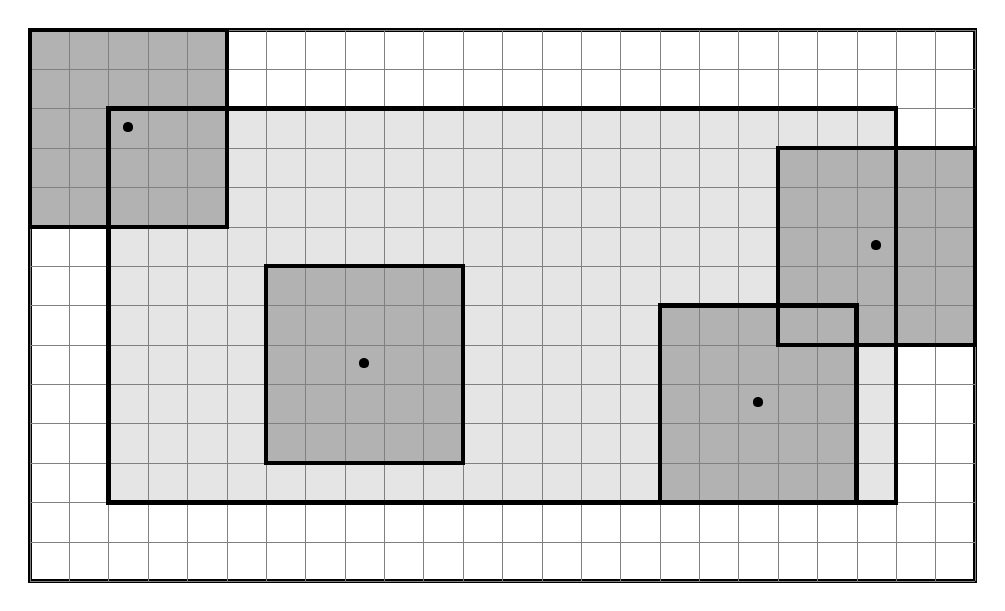
\begin{tikzpicture}
\node[draw, minimum width=12cm, minimum height=
    7cm, ultra thick](outer_rec)[]{};
\node[draw, minimum width=10cm, minimum height=
    5cm, ultra thick, fill=black!10!](inner_rec)[]{};
\node[draw, minimum width=2.5cm, minimum height=2.5cm,
    ultra thick, fill=black!30!](square1)at(-4.75,2.25){\textbullet};
\node[draw, minimum width=2.5cm, minimum height=2.5cm,
    ultra thick,fill=black!30!](square2)at(-1.75,-.75){\textbullet};
\node[draw, minimum width=2.5cm, minimum height=2.5cm,
    ultra thick, fill=black!30!](square3)at(4.75,.75){\textbullet};
\node[draw, minimum width=2.5cm, minimum height=2.5cm,
    ultra thick, fill=black!30!](square4)at(3.25,-1.25){\textbullet};
\draw[step=.5, ultra thin, color=black!50!](-6,-3.5)grid(6,3.5);

%redraw borders
\node[draw, minimum width=10cm, minimum height=
    5cm, ultra thick, ][]{};
\node[draw, minimum width=2.5cm, minimum height=2.5cm,
    ultra thick]at(-4.75,2.25){};
\node[draw, minimum width=2.5cm, minimum height=2.5cm,
    ultra thick]at(-1.75,-.75){};
\node[draw, minimum width=2.5cm, minimum height=2.5cm,
    ultra thick]at(4.75,.75){};
\node[draw, minimum width=2.5cm, minimum height=2.5cm,
    ultra thick]at(3.25,-1.25){};
\end{tikzpicture}
\caption{This diagram illustrates how to convolve an image with a filter.
The light grey rectangle represents the original image $A$, and the dark grey squares are the filter $F$.
The larger rectangle is the image padded with zeros; i.e., all pixel values in the outer white band are 0.
To compute the entry of the convolution matrix $C$ located at a black dot, take the inner product of $F$ with the submatrix of the padded image centered at the dot.}
\label{fig:convolution}
\end{figure}

\subsubsection*{Implementation in NumPy} % - - - - - - - - - - - - - - - - - -

Let us write a function that convolves an image with a filter.
You can test this function on the image \li{cameraman.jpg}, which appears in Figure \ref{fig:cameraman}.
The following code loads this image and plots it with matplotlib.

\begin{lstlisting}
>>> image = plt.imread('cameraman.jpg')
>>> plt.imshow(image, cmap = 'gray')
>>> plt.show()
\end{lstlisting}

Here is the function definition and some setup.

\begin{lstlisting}
1. def Filter(image, F):
2.     m, n = image.shape
3.     h, k = F.shape
\end{lstlisting}

To convolve \li{image} with the filter \li{F}, we must first \emph{pad} the array \li{image} with zeros around the edges.
This is because in \eqref{equ:convolve}, entries $A_{ij}$ are set to zero when $i$ or $j$ is out of bounds.
We do this by creating a larger array of zeros, and then making the interior part of the array equal to the original image (see Figure \ref{fig:convolution}).

For example, if the filter is a $3 \times 3$ matrix, then the following code will pad the matrix with the appropriate number of zeros.

\begin{lstlisting}
 # Create a larger matrix of zeros
image_pad = np.zeros((m+2, n+2))
# Make the interior of image_pad equal to the original image
image_pad[1:1+m, 1:1+n] = image
\end{lstlisting}

We want to do this in general in our function.  Note that the number of zeros we need to pad our array depends on the size of the filter \li{F}.

\begin{lstlisting}
5.    image_pad = # Create an array of zeros of the appropriate size
6.   # Make the interior of image_pad equal to image
\end{lstlisting}

Finally, we iterate through the image to compute each entry of the convolution matrix.

\begin{lstlisting}
7.    C = np.zeros(image.shape)
8.    for i in range(m):
9.        for j in range(n):
10.            C[i,j] = # Compute C[i, j]
\end{lstlisting}

\subsubsection*{Gaussian Blur} % - - - - - - - - - - - - - - - - - - - - - - -

A \emph{Gaussian blur} is an image filter that operates on an image by convolving with the matrix
\[
G = \frac{1}{159}\begin{pmatrix}
2&4&5&4&2\\
4&9&12&9&4\\
5&12&15&12&5\\
4&9&12&9&4\\
2&4&5&4&2
\end{pmatrix}.
\]

Blurring an image can remove ``noise'', or random variation that is the visual analog of static in a radio signal (and equally undesirable).

\begin{problem}\label{prob:filter}
\leavevmode
Finish writing the function \li{Filter} by filling in lines 5, 6, and 10.  Hint: Note in \ref{equ:convolve}, $C_{ij}$ was calculated by summing from -1 to 1.  This is only the case if the filter \li{F} is $3 \times 3$. A slight modification is needed in the general case.  Test your function on the image \li{cameraman.jpg} using the Gaussian Blur. The result is in Figure \ref{fig:cameraman_blur}.
\end{problem}

% TODO: make pictures that aren't pdfs
\begin{figure}
\centering
\begin{subfigure}[b]{.49\textwidth}
\centering
\includegraphics[width=\textwidth]{figures/cameraman.jpg}
\caption{Unfiltered image.}
\label{fig:cameraman}
\end{subfigure}
\begin{subfigure}[b]{.49\textwidth}
\centering
\includegraphics[width=\textwidth]{figures/cameramanBlur.pdf}
\caption{Image after Gaussian blur is applied.}
\label{fig:cameraman_blur}
\end{subfigure}
\begin{subfigure}[b]{.49\textwidth}
\centering
\includegraphics[width=\textwidth]{figures/edges.pdf}
\caption{Image after the Sobel filter is applied.}
\label{fig:cameraman_edges}
\end{subfigure}
\caption{Here is an example of a Gaussian blur and the Sobel filter applied to an image.
This photo, known as ``cameraman,'' is a standard test image in image processing.
A database of such images can be downloaded from \url{http://www.imageprocessingplace.com/root_files_V3/image_databases.htm}.}
\label{fig:cameraman1}
\end{figure}

\subsection*{Edge Detection} % ------------------------------------------------

Automatic detection of edges in an image can be used to segment or sharpen the image.
We will find edges with the Sobel filter, which computes the gradient of the image at each pixel.
The magnitude of the gradient tells us the rate of change of the pixel values, and so large magnitudes should
correspond to edges within the image.
The Sobel filter is not a convolution, although it does use convolutions.

We can think of an image as a function from a $2 \times 2$ grid of points to $\mathbb{R}$.
The image maps a pixel location to an intensity.
It does not make sense to define the derivative of this function as a limit because the domain is discrete---a step size $h$ cannot take on arbitrarily small values.
Instead, we \emph{define} the derivative to be the centered difference quotient of the previous section.
That is, we define the derivative in the $x$-direction at the $ij^{th}$ pixel to be
\[
\frac{1}{2}A_{i+1, j} - \frac{1}{2}A_{i-1, j}.
\]

We can use a convolution to create a matrix $A_x$ whose $ij^{th}$ entry is the derivative of $A$ at the $ij^{th}$ entry, in the $x$-direction.
In fact, $A_x = A \ast S$, where
\[
S = \frac{1}{8}
\left[\begin{array}{ccc}
-1 & 0 & 1\\
-2 & 0 & 2\\
-1 & 0 & 1
\end{array}\right].
\]

Note that this convolution takes a weighted average of the $x$-derivatives at $(i, j)$, $(i, j+1)$, and $(i, j-1)$.
The derivative at $(i, j)$ is weighted by 2.
Using a weighted average instead of just the derivative at $(i, j)$ makes the derivative less affected by noise.

Now we can define the Sobel filter.
A Sobel filter applied to an image $A$ results in an array $B = (B_{ij})$ of 0's and 1's, where the 1's trace out the edges in the image.
By definition,
\[
B_{ij} = \left\{
     \begin{array}{ll}
       1 & \text{if}\; \;\|\nabla A(ij)\|_2 > M \\
       0 & \text{otherwise}.
     \end{array}
   \right.
\]
Here, $\nabla A(ij) = ((A \ast S)_{ij}, (A\ast S^T)_{ij})$ is the gradient of $A$ at the $ij^{th}$ pixel.
The constant $M$ should be ``sufficiently large'' enough to pick out those pixels with the largest gradient (i.e., those pixels that are part of an edge).
A good choice for $M$ is 4 times the average value of $\|\nabla A(ij)\|_2$ over the whole image $A$.

When the Sobel filter is applied to \li{cameraman.jpg}, we get the image in Figure \ref{fig:cameraman_edges}.
Here, the 1's in $B$ were mapped to ``white'' and the 0's were mapped to ``black.''

\begin{problem}
Write a function that accepts an image as input and applies the Sobel filter to the image.  Test your function on \li{cameraman.jpg}.  Hint: If you want to find the average of a matrix \li{A}, use the function \li{A.mean()}.
\end{problem}
\end{comment}
